\reportheading{2.\quad 研究方法}
两项任务均采用 Fire Dynamics Simulator 6.10.1（FDS）~\cite{fdsuser}。丙烷火沿用实验条件，用实测顶棚温升检验模型。丙烯火设计加入烟炱生成、顶棚机械排烟及补风，考察这些条件下房间能保有多少净高。

\reportfigure{\resizebox{.92\linewidth}{!}{\begin{tikzpicture}[font=\sffamily\large,text=ink,
 labelnode/.style={align=center,inner sep=3pt},
 title/.style={font=\sffamily\bfseries\large,align=center,inner xsep=9pt,inner ysep=3pt},
 flow/.style={draw=ink!85,line width=.85pt,-{Stealth[length=1.55mm]},rounded corners=2pt},
 stage/.style={draw=sea,line width=1.25pt,-{Stealth[length=1.75mm]}},
 tag/.style={font=\sffamily\normalsize,inner sep=2pt}]
% The stage bands carry the sequence; illustrations belong to their own stage.
\filldraw[draw=sea!30,fill=sea!6] (0,0) rectangle (15,-2.08);
\filldraw[draw=sea!30,fill=sea!4] (0,-2.94) rectangle (15,-5.05);
\filldraw[draw=ochre!40,fill=ochre!6] (0,-5.91) rectangle (15,-14.30);
\node[title,fill=sea!18] at (7.5,0) {房间与火源参数};
\node[title,fill=sea!18] at (7.5,-2.94) {任务 1\quad 丙烷火验证};
\node[title,fill=ochre!21] at (7.5,-5.91) {任务 2\quad 丙烯火排烟设计与优化};
\draw[stage] (7.5,-2.12)--(7.5,-2.61);
\draw[stage] (7.5,-5.09)--(7.5,-5.58);
% Physical plan and door states, simplified from the report's layout.
\begin{scope}[shift={(.66,-1.18)},x=.52cm,y=.52cm]
\filldraw[draw=ink,fill=white,thick] (0,0) rectangle (6.6,.9);
\foreach \x in {.825,2.475,4.125,5.775}
 \draw[sea,line width=2pt] (\x-.215,.9)--(\x+.215,.9);
\fill[clay] (3.175,.325) rectangle (3.425,.575);
\end{scope}
\node[labelnode] at (2.38,-1.66) {房间长度 6.60 m};
\foreach \y/\id in {-.74/OP-1,-1.16/OP-6}{
 \node[anchor=east,font=\sffamily\normalsize] at (6.83,\y) {\id};
 \foreach \k in {0,...,3}{\draw[ink!65,fill=white] (7+.42*\k,\y-.1) rectangle ++(.28,.20);}
}
\foreach \k in {0,...,3}{\fill[sea] (7+.42*\k,-.84) rectangle ++(.28,.20);}
\fill[sea] (7+.42*2,-1.26) rectangle ++(.28,.20);
\node[labelnode] at (7.50,-1.66) {侧门开启状态};
% Two burner symbols indicate the two prescribed heat release rates.
\foreach \x/\s in {11.73/.68,12.82/1}{
 \begin{scope}[shift={(\x,-1.24)},scale=\s]
 \draw[ink,line width=1.2pt] (-.31,0)--(.31,0);
 \fill[clay] (0,.04).. controls (-.53,.17) and (-.13,.51) ..(-.10,.65)
 .. controls (.05,.53) and (.11,.42) ..(.14,.30)
 .. controls (.23,.45) and (.23,.47) ..(.24,.52)
 .. controls (.50,.18) and (.26,.06) ..(0,.04);
 \end{scope}}
\node[labelnode] at (12.32,-1.66) {47.2 / 106.2 kW};
% Centre thumbnail uses the actual paired profile for OP-1 at 106.2 kW.
\begin{scope}[shift={(1.57,-4.21)},x=.33cm,y=.21cm]
\draw[step=1,sea!65,thin] (0,0) grid (5,2);
\draw[ink] (0,0) rectangle (5,2);
\draw[ink] (0,2)--(.7,2.85)--(5.7,2.85)--(5,2) (5.7,2.85)--(5.7,.85)--(5,0);
\end{scope}
\node[labelnode] at (2.52,-4.64) {运行四组 FDS};
\begin{axis}[at={(6.43cm,-4.25cm)},anchor=south west,scale only axis,width=2.08cm,height=.77cm,
 axis lines=left,axis line style={-,ink!55},xtick=\empty,ytick=\empty,xmin=0,xmax=660,ymin=250,ymax=1000]
\addplot[sea,thick] table[col sep=comma,x=sensor_x_cm,y=fds_rise_K]{../../05_Calculations/op1_106_coarse_90_120.csv};
\addplot[clay,only marks,mark=*,mark size=.85pt] table[col sep=comma,x=sensor_x_cm,y=exp_rise_K]{../../05_Calculations/op1_106_coarse_90_120.csv};
\end{axis}
\node[labelnode] at (7.48,-4.64) {对照 51 个测点};
\node[labelnode] at (12.45,-4.12) {比较不同门态下的\\峰值与温度剖面};
\draw[flow] (4.52,-4.07)--(5.59,-4.07);
\draw[flow] (9.33,-4.07)--(10.39,-4.07);

% The left lane follows physical design decisions. The right lane analyses FDS records.
\tikzset{designnode/.style={labelnode,font=\sffamily\small},
 decision/.style={designnode,draw=ochre!80,fill=white,rounded corners=2pt,inner sep=4pt}}
\draw[ochre!32] (8.42,-6.35)--(8.42,-13.97);
\node[designnode] (initial) at (2.23,-6.98) {\textbf{16 个 OP-6 方案}\\达标数 0/16};
\node[designnode] (layout) at (6.28,-6.98) {\textbf{调整布局}\\垂壁、排烟与补风};
\draw[flow] (initial.east)--(layout.west);
\node[designnode] (coarse) at (6.28,-8.47) {\textbf{FDS 粗网格筛选}\\0.96、1.28 通过};
\draw[flow] (layout.south)--(coarse.north);
\node[designnode] (refine) at (2.23,-8.47) {\textbf{加密竖向网格}\\复查净高};
\draw[flow] (coarse.west)--(refine.east);
\node[decision] (gate) at (2.23,-10.05) {\textbf{测试 1.12}\\OP-6，烟炱产率 0.02};
\draw[flow] (refine.south)--(gate.north);
\node[designnode] (six) at (6.28,-10.05) {\textbf{复核 1.12}\\两种门态，三种产率};
\draw[flow] (gate.east)--(six.west);
\node[designnode] (verified) at (2.23,-11.85) {\textbf{八个测柱，120 s}\\$h_{\min}=0.4358$ m};
\draw[flow] (six.south)--(six.south |- verified.east)--(verified.east);
\node[designnode,fill=white,draw=ochre!55,inner sep=5pt] (power) at (4.16,-13.42)
 {$\displaystyle\min P$\quad s.t.\ 各测点净高 $\geq0.38$ m\\
 \textbf{选择 1.12 m$^3$/s}\quad 6.91 W；1.28 为 10.32 W};
\draw[flow] (verified.south)--(verified.south |- power.north);
\node[designnode,text=sea] (replay) at (11.82,-6.67) {\textbf{回放同组 16 个方案}};
\draw[flow] (initial.north)--++(0,.30)-|(8.72,-6.67)--(replay.west);
\foreach \x/\heading/\ranks in {
 10.25/{贝叶斯优化}/{1,9,12,2,10,16,5,11,14,6,15,7,3,13,8,4},
 13.22/{遗传算法}/{1,13,8,2,14,10,9,5,15,16,7,6,3,12,11,4}}{
 \node[align=center,font=\sffamily\normalsize] at (\x,-7.36) {\heading};
 \foreach \q [count=\i from 0] in \ranks{
  \pgfmathtruncatemacro{\rownum}{int(\i/4)}
  \pgfmathtruncatemacro{\colnum}{mod(\i,4)}
  \begin{scope}[shift={(\x+.42*\colnum-.63,-7.99-.34*\rownum)}]
   \ifnum\i=11
    \fill[sea] (-.21,-.17) rectangle (.21,.17);
    \node[text=white,font=\sffamily\bfseries\small] {\q};
   \else
    \filldraw[draw=ink!24,fill=white,line width=.3pt] (-.21,-.17) rectangle (.21,.17);
    \node[font=\sffamily\small] {\q};
   \fi
  \end{scope}}
}

\node[designnode] at (11.82,-9.83) {查到最大余量\\固定 16 \quad BO 7 \quad GA 6--11};
\node[designnode] (hist) at (11.82,-11.04) {\textbf{已归档 FDS 最低净高}};
\node[designnode] (pred) at (11.82,-12.18) {\textbf{PINN 与回归}\\预测候选方案最低净高};
\node[designnode,text=sea] (test) at (11.82,-13.53) {以留出 FDS 结果\\检验预筛精度};
\draw[flow] (hist.south)--(pred.north);
\draw[flow] (pred.south)--(test.north);
\draw[flow,draw=sea] (pred.west)--(8.80,-12.18)--node[pos=.48,above,sloped,font=\sffamily\small,text=sea]{建议检查顺序}(8.80,-8.47)--(coarse.east);
\end{tikzpicture}
}}{左栏为 FDS 筛选和风量决策。右栏为两项独立分析：BO/GA 回放设计顺序，代理模型预估工况最低净高。风量单位为 m$^3$/s。蓝绿色单元格标出回放中净高余量最大的方案（GA 示意采用随机种子 0）。回箭头表示可用代理模型安排未来 FDS 的检查顺序。}


\subhead{2.1\quad 任务 1：丙烷火与顶棚射流验证}
房间尺寸取自题目 B 任务书图 1 和 Peng 等的实验~\cite{peng}。模型内部长、宽、高分别为 $6.60\times0.90\times0.76$~m，地面正中的正方形燃烧器边长 0.25~m，中心位于 $x=3.30$~m。同一侧墙上设四个门洞，沿 $x$ 递增方向依次为 L2、L1、R1 和 R2，各宽 0.43~m、高 0.63~m。计算域从这面墙向外延伸至 $y=1.40$~m，使空气可以从同一门洞的不同高度进出。参考环境温度为 $27.5\,^{\circ}$C。

第 18 组在四门全开（OP-1）和仅开 R1（OP-6）时，各自计算 47.2 和 106.2~kW 两档名义热释放率。FDS 按单位燃烧器面积指定热释放率，燃烧器边缘对齐网格面后，实际占地面积可能随网格改变。因此，每次换网格都核对燃烧器面积，并检查计算中记录的热释放率。

\clearpage
\subhead{空间分辨率与物理子模型}
OP-1 在相同计算域中采用 $132\times28\times19$、$176\times36\times25$ 和 $220\times48\times32$ 三种网格。按 FDS 用户指南~\cite{fdsuser}，火源特征直径为
\[
 D^*=\left(\frac{\dot Q}{\rho_\infty c_p T_\infty\sqrt{g}}\right)^{2/5}.
\]
式中 $\dot Q$ 为名义火源功率，$g$ 为重力加速度，$\rho_\infty$、$c_p$ 和 $T_\infty$ 分别为环境空气的密度、比热容和绝对温度。以 $D^*$ 除以单元最长边，可比较各网格对火源的分辨能力。再对照各网格算出的纵向温升剖面，判断加密对结果的影响。

\subhead{任务 1：控制变量对照与实验测量}
在 OP-1、106.2~kW 的粗网格上，先将辐射份额固定为 0.29，比较 Deardorff 与 WALE 两种亚网格模型~\cite{fdstech}。Yuen 等也在房间火灾模拟中考察过模型选择的影响~\cite{yuen}。随后保留 Deardorff，将辐射份额分别调至 0.20 和 0.50。壁面散热另作成对比较，将绝热壁换成 15~mm 导热板。板厚取自 Peng 等的实验~\cite{peng}，密度 200~kg/m$^3$、导热系数 0.10~W/(m\,K) 和比热容 1.0~kJ/(kg\,K) 则借用 FDS Steckler 第 10 号算例的保温材料参数~\cite{steckler}。OP-6 的两种壁面均用 $154\times56\times23$ 门流诊断网格。47.2~kW 的 OP-1 对照均用原粗网格。

从 Peng 等~\cite{peng}图 9 的顶棚纵向温升曲线读取 51 个位置，与模型中 $z=0.74$~m 处的 1~mm 热电偶逐点配对。对位置 $i$，按设备实际输出间隔求 90--120~s 内的时间加权平均温度，再减去模型环境温度，即得该点的模拟温升。取 $e_i=\Delta T_{\mathrm{FDS},i}-\Delta T_{\mathrm{exp},i}$，则整条剖面的平均偏差和均方根误差分别为
\[
 \mathrm{bias}=\frac{1}{51}\sum_{i=1}^{51}e_i,\qquad
 \mathrm{RMSE}=\sqrt{\frac{1}{51}\sum_{i=1}^{51}e_i^2}.
\]
另记录最热测点相对燃烧器中心的位置，以判断峰位是否偏移。同一时段内，R1 门口的速度和温度剖面给出各高度的进出流向和气流温度。将门流结果与壁面、辐射对照结合，可分析门洞输运与围护结构散热对顶棚温升的影响。

\subhead{房间平面与排烟布局}
\reportfigure{\begin{tikzpicture}[x=1.52cm,y=1.52cm,font=\sffamily\footnotesize]
\fill[teal!5] (0,0) rectangle (6.6,.9);
\draw[ink,line width=.7pt] (0,0) rectangle (6.6,.9);
\foreach \x/\id in {.825/L2,2.475/L1,4.125/R1,5.775/R2}{
 \draw[white,line width=2.3pt] (\x-.215,.9)--(\x+.215,.9);
 \draw[teal,line width=2pt] (\x-.215,.9)--(\x+.215,.9);
 \node[above,text=teal] at (\x,1.01){\bfseries \id};}
\filldraw[fill=teal!24,draw=teal] (2.9,.05) rectangle (3.3,.85);
\filldraw[fill=teal!24,draw=teal] (3.3,.05) rectangle (3.7,.85);
\foreach \x in {2.8,3.8}{\draw[ink,dashed,thick] (\x,0)--(\x,.9);}
\filldraw[fill=rust!30,draw=rust] (3.175,.325) rectangle (3.425,.575);
\foreach \x in {0,6.6}{\draw[teal,line width=2.4pt] (\x,0)--(\x,.9);}
\draw[gray!70,|<->|] (0,-.22)--node[fill=white,inner sep=2pt,text=ink]{6.60 m}(6.6,-.22);
\draw[gray!70,|<->|] (6.90,0)--(6.90,.9);
\node[right,text=ink] at (6.92,.45){0.90 m};
\end{tikzpicture}\par
{\sffamily\footnotesize\textcolor{rust}{\rule{6pt}{6pt}} 燃烧器\qquad
\textcolor{teal!65}{\rule{6pt}{6pt}} 顶棚排烟口\qquad
\textcolor{ink}{-- --} 挡烟垂壁\qquad\textcolor{teal}{\rule[.4ex]{10pt}{1.6pt}} 开口}}{名义几何的平面图。丙烷火模型使用图示侧开口。丙烯火设计增加端墙补风口，并在燃烧器上方两道挡烟垂壁之间设置两个顶棚排烟口。}

\clearpage
\subhead{2.2\quad 任务 2：丙烯火与排烟设计}
丙烯火的名义热释放率为 106.2~kW。基准烟炱产率取 0.02~kg/kg 燃料，CO 产率取 0.01~kg/kg。另将烟炱产率提高至 0.05 和 0.10~kg/kg，CO 产率保持原值。每种烟炱产率分别计算 OP-1 和 OP-6，共六个工况，每次计算中门的开闭状态固定。原设计网格为 $132\times28\times19$，围护结构表面按绝热处理。

\subhead{候选方案筛选与布局调整}
两次回放回答不同的检查次序问题。原布局中，BO 和 GA 根据此前查到的 FDS 余量选择下一个设计。改进布局中，PINN 等模型根据已有 FDS 数据预测最低净高，决定同一风量下先查哪个工况。最终选取风量时，逐一核查六个工况的完整 FDS 记录。

最初在 OP-6、基准烟炱产率下，将四种挡烟垂壁下垂深度（0、0.08、0.16、0.24~m）与四种总排烟量（0.08、0.16、0.24、0.32~m$^3$/s）交叉组合。固定顺序、贝叶斯优化（BO）~\cite{bo} 和遗传算法（GA）~\cite{ga} 均从同样的四个角点设计开始。每次查询揭示一个已归档的 FDS 余量，BO 和 GA 仅使用当时已揭示的余量选择下一设计。统计首次发现最大已记录余量所需的全部查询次数，GA 使用 20 个随机种子重复回放。

改进布局从两侧端墙的近地面开口补风。开口下缘与地面齐平，OP-1 时开至 0.44~m，OP-6 时开至 0.48~m。燃烧器正上方设两个顶棚排烟口，各接一条独立支管。两道横向挡烟垂壁位于排烟口两侧，分别设在 $x=2.8$ 和 3.8~m 处，自顶棚下垂 0.24~m。

\reportfigure{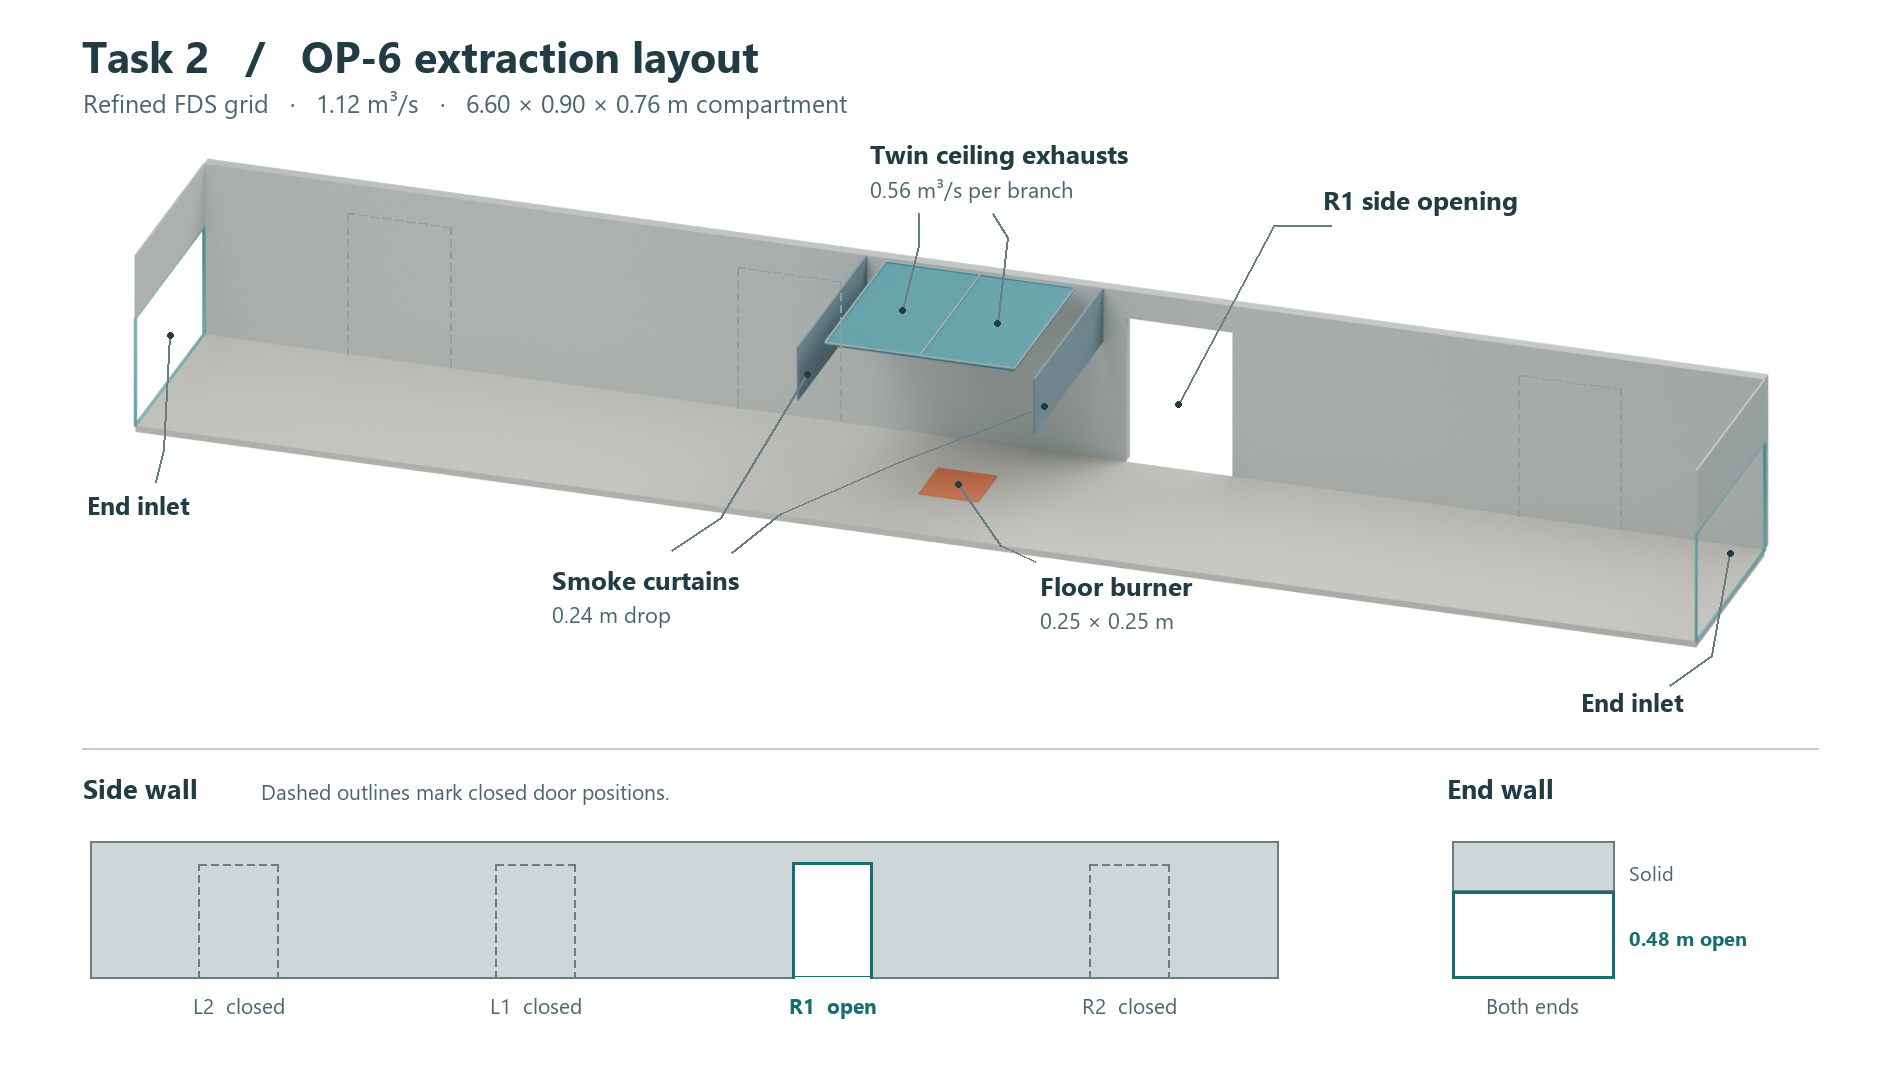
\includegraphics[width=\linewidth]{../figures/op6_1p12_fds_geometry_review.png}}{OP-6 改进布局的细网格剖视图。为展示室内构件，图中剖去近侧墙。FDS 中该处（$y=0$）为连续绝热墙面。侧墙只开启 R1，虚线标出关闭的三个门位。两端墙各设一个从地面起高 0.48~m 的补风口。}

按上述高度设置补风口，两条排烟支管均分总风量。先在六个工况下比较 0.96 和 1.28~m$^3$/s，再加密竖向网格，测试中间一档 1.12~m$^3$/s。另作工况排序回放时，将上述补风布局整类留出，不参与训练。物理信息神经网络（PINN）在拟合观测数据时可加入物理方程的残差约束~\cite{pinn}。三个风量按功率递增检查，每个风量下按 PINN、直接回归或二者等权平均预测的净高排序，先查预测最低的工况（第 5.2 节）。

\subhead{烟层高度判据与局部烟气测量}
FDS 在中央纵剖面 $y=0.45$~m 上布置八列竖向测点，根据温度推算烟层高度 $h_j(t)$。沿房间纵向的位置为 0.5、1.7、2.4、3.0、3.6、4.2、4.9 和 6.1~m。设备名义采样间隔为 0.5~s。工况 $s$ 的采样净高余量为
\[
 m_s=\min_{j,\,0\leq t\leq120\,\mathrm{s}} h_{j,s}(t)-0.38\,\mathrm{m}.
\]
净高阈值取房间半高。筛选时，只要一个测点在一个时刻低于阈值，就可以判定该方案越限。其余候选方案须查完六个工况各自 120~s 的记录。八列测点中余量最小的那一条记录，给出控制净高的门态、烟炱产率、位置和时刻。

\subhead{任务 2：光学条件、CO 与风机功率}
在这八个纵向位置另设半高探头（$z=0.38$~m），记录能见度和 CO 体积分数。中央纵剖面的消光系数分布用于查看火源附近和远端的烟气。净高按温度分层判断，半高探头则给出该位置的局部暴露。CO 生成量按燃料消耗量和指定产率估算，到达测点的浓度还受输运、稀释和排出的影响。比较设计时同时核对实际火源功率。

总排烟量 $Q$ 由两条短支管均分时，估算总输入电功率为
\[
 P_{\mathrm{el}}=\frac{Q\,\Delta p}{\eta},\qquad
 \Delta p=\left(f\frac{L}{D_h}+K\right)\frac{\rho}{2}
                 \left(\frac{Q}{2A}\right)^2 .
\]
每条短支管的截面积为 $A=0.32$~m$^2$，长度为 $L=0.40$~m。计算取水力直径 $D_h=0.533$~m、空气密度 $\rho=1.2$~kg/m$^3$、达西摩阻系数 $f=0.02$ 和局部阻力系数 $K=2$。两支管并联，每条承担一半风量，压降相同。按风机效率 $\eta=0.60$ 计算两支管合计所需电功率。实际选风机时，还需计入全系统压损并查风机性能曲线。

\subhead{设计风量的选取与复核}
选取排烟量时，保持水平网格、补风口及挡烟垂壁不变，将竖向单元从 19 层加至 38 层，并测试原有两档之间的风量 1.12~m$^3$/s。图 4(b) 对比 OP-6、基准烟炱产率在同一加密网格上的三档结果。所选风量能否满足要求，再按两种门态、三种烟炱产率逐一检查各工况的八测柱记录，每组覆盖 120~s（表 D3）。

\clearpage
\subhead{2.3\quad 排烟系统的约束优化}
任务书指定最低净高，并要求估算机械排烟功率。第 18 组选择所需风机输入电功率最小作为设计目标。记 $g$ 为候选布局，$Q$ 为总排烟量（m$^3$/s），$P$ 为所需输入电功率（W），则优化问题写为
\begin{equation}
\begin{aligned}
\min_{g,Q,P}\quad &P\\
\mathrm{s.t.}\quad
 &h_{s,i,t}(g,Q)\geq 0.38\,\mathrm{m}
       &&\forall s\in S,\ i\in I,\ t\in T_s,\\
 &P\geq Q\,\Delta p_s(g,Q)/\eta_s(g,Q)
       &&\forall s\in S,\\
 &g\in G,\quad Q\in\mathcal Q(g),\quad P\geq0 .
\end{aligned}
\label{eq:design}
\end{equation}
$G$ 为排烟口、挡烟垂壁与补风口布局的候选集合。各门态下的补风口预设属于 $g$ 的一部分，在该门态的各烟炱产率下通用。所有工况共用同一个 $Q$，从该布局已测试的风量集合 $\mathcal Q(g)$ 中选取。$S$ 包含两种门态和三种烟炱产率组成的六个工况。$I$ 为八个测点的位置集合，$T_s$ 为工况 $s$ 的完整 120~s 模拟中设备记录的时刻集合。第一项约束检验每个测点和时刻。第二项按全部工况中的最大功率需求确定输入功率，其中压降 $\Delta p_s$ 的单位为 Pa，总效率满足 $0<\eta_s\leq1$。

目标函数中的功率按第 2.2 节的两条短支管损失估算。对已测候选方案逐一计算最不利采样余量，
\[
m(g,Q)=\min_{s\in S,\ i\in I,\ t\in T_s}
           \{h_{s,i,t}(g,Q)-0.38\,\mathrm{m}\}.
\]
逐一比较满足 $m\geq0$ 的候选方案，选取其中估算电功率最低者。第 5.2 节回放原布局的筛选过程，以首次找到最大已记录余量所需的查询次数，比较 BO、GA 和固定顺序。
